\PassOptionsToPackage{unicode=true}{hyperref} % options for packages loaded elsewhere
\PassOptionsToPackage{hyphens}{url}
%
\documentclass[
  a4paper,
]{article}



\usepackage{lmodern}
\usepackage{amssymb,amsmath}
\usepackage{ifxetex,ifluatex}
\ifnum 0\ifxetex 1\fi\ifluatex 1\fi=0 % if pdftex
  \usepackage[T1]{fontenc}
  \usepackage[utf8]{inputenc}
  \usepackage{textcomp} % provides euro and other symbols
\else % if luatex or xelatex
  \usepackage{unicode-math}
  \defaultfontfeatures{Scale=MatchLowercase}
  \defaultfontfeatures[\rmfamily]{Ligatures=TeX,Scale=1}
\fi
% use upquote if available, for straight quotes in verbatim environments
\IfFileExists{upquote.sty}{\usepackage{upquote}}{}
\IfFileExists{microtype.sty}{% use microtype if available
  \usepackage[]{microtype}
  \UseMicrotypeSet[protrusion]{basicmath} % disable protrusion for tt fonts
}{}
\makeatletter
\@ifundefined{KOMAClassName}{% if non-KOMA class
  \IfFileExists{parskip.sty}{%
    \usepackage{parskip}
  }{% else
    \setlength{\parindent}{0pt}
    \setlength{\parskip}{6pt plus 2pt minus 1pt}}
}{% if KOMA class
  \KOMAoptions{parskip=half}}
\makeatother
\usepackage{xcolor}
\IfFileExists{xurl.sty}{\usepackage{xurl}}{} % add URL line breaks if available
\IfFileExists{bookmark.sty}{\usepackage{bookmark}}{\usepackage{hyperref}}
\hypersetup{
  pdftitle={Design of Sensor Signal Processing with ForSyDe},
  pdfborder={0 0 0},
  breaklinks=true}
\urlstyle{same}  % don't use monospace font for urls
\usepackage{color}
\usepackage{fancyvrb}
\newcommand{\VerbBar}{|}
\newcommand{\VERB}{\Verb[commandchars=\\\{\}]}
\DefineVerbatimEnvironment{Highlighting}{Verbatim}{commandchars=\\\{\}}
% Add ',fontsize=\small' for more characters per line
\newenvironment{Shaded}{}{}
\newcommand{\AlertTok}[1]{\textcolor[rgb]{1.00,0.00,0.00}{\textbf{#1}}}
\newcommand{\AnnotationTok}[1]{\textcolor[rgb]{0.38,0.63,0.69}{\textbf{\textit{#1}}}}
\newcommand{\AttributeTok}[1]{\textcolor[rgb]{0.49,0.56,0.16}{#1}}
\newcommand{\BaseNTok}[1]{\textcolor[rgb]{0.25,0.63,0.44}{#1}}
\newcommand{\BuiltInTok}[1]{#1}
\newcommand{\CharTok}[1]{\textcolor[rgb]{0.25,0.44,0.63}{#1}}
\newcommand{\CommentTok}[1]{\textcolor[rgb]{0.38,0.63,0.69}{\textit{#1}}}
\newcommand{\CommentVarTok}[1]{\textcolor[rgb]{0.38,0.63,0.69}{\textbf{\textit{#1}}}}
\newcommand{\ConstantTok}[1]{\textcolor[rgb]{0.53,0.00,0.00}{#1}}
\newcommand{\ControlFlowTok}[1]{\textcolor[rgb]{0.00,0.44,0.13}{\textbf{#1}}}
\newcommand{\DataTypeTok}[1]{\textcolor[rgb]{0.56,0.13,0.00}{#1}}
\newcommand{\DecValTok}[1]{\textcolor[rgb]{0.25,0.63,0.44}{#1}}
\newcommand{\DocumentationTok}[1]{\textcolor[rgb]{0.73,0.13,0.13}{\textit{#1}}}
\newcommand{\ErrorTok}[1]{\textcolor[rgb]{1.00,0.00,0.00}{\textbf{#1}}}
\newcommand{\ExtensionTok}[1]{#1}
\newcommand{\FloatTok}[1]{\textcolor[rgb]{0.25,0.63,0.44}{#1}}
\newcommand{\FunctionTok}[1]{\textcolor[rgb]{0.02,0.16,0.49}{#1}}
\newcommand{\ImportTok}[1]{#1}
\newcommand{\InformationTok}[1]{\textcolor[rgb]{0.38,0.63,0.69}{\textbf{\textit{#1}}}}
\newcommand{\KeywordTok}[1]{\textcolor[rgb]{0.00,0.44,0.13}{\textbf{#1}}}
\newcommand{\NormalTok}[1]{#1}
\newcommand{\OperatorTok}[1]{\textcolor[rgb]{0.40,0.40,0.40}{#1}}
\newcommand{\OtherTok}[1]{\textcolor[rgb]{0.00,0.44,0.13}{#1}}
\newcommand{\PreprocessorTok}[1]{\textcolor[rgb]{0.74,0.48,0.00}{#1}}
\newcommand{\RegionMarkerTok}[1]{#1}
\newcommand{\SpecialCharTok}[1]{\textcolor[rgb]{0.25,0.44,0.63}{#1}}
\newcommand{\SpecialStringTok}[1]{\textcolor[rgb]{0.73,0.40,0.53}{#1}}
\newcommand{\StringTok}[1]{\textcolor[rgb]{0.25,0.44,0.63}{#1}}
\newcommand{\VariableTok}[1]{\textcolor[rgb]{0.10,0.09,0.49}{#1}}
\newcommand{\VerbatimStringTok}[1]{\textcolor[rgb]{0.25,0.44,0.63}{#1}}
\newcommand{\WarningTok}[1]{\textcolor[rgb]{0.38,0.63,0.69}{\textbf{\textit{#1}}}}
\usepackage{longtable,booktabs}
% Allow footnotes in longtable head/foot
\IfFileExists{footnotehyper.sty}{\usepackage{footnotehyper}}{\usepackage{footnote}}
\makesavenoteenv{longtable}
\usepackage{graphicx,grffile}
\makeatletter
\def\maxwidth{\ifdim\Gin@nat@width>\linewidth\linewidth\else\Gin@nat@width\fi}
\def\maxheight{\ifdim\Gin@nat@height>\textheight\textheight\else\Gin@nat@height\fi}
\makeatother
% Scale images if necessary, so that they will not overflow the page
% margins by default, and it is still possible to overwrite the defaults
% using explicit options in \includegraphics[width, height, ...]{}
\setkeys{Gin}{width=\maxwidth,height=\maxheight,keepaspectratio}
\setlength{\emergencystretch}{3em}  % prevent overfull lines
\providecommand{\tightlist}{%
  \setlength{\itemsep}{0pt}\setlength{\parskip}{0pt}}
\setcounter{secnumdepth}{5}
% Redefines (sub)paragraphs to behave more like sections
\ifx\paragraph\undefined\else
  \let\oldparagraph\paragraph
  \renewcommand{\paragraph}[1]{\oldparagraph{#1}\mbox{}}
\fi
\ifx\subparagraph\undefined\else
  \let\oldsubparagraph\subparagraph
  \renewcommand{\subparagraph}[1]{\oldsubparagraph{#1}\mbox{}}
\fi

% set default figure placement to htbp
\makeatletter
\def\fps@figure{htbp}
\makeatother

\usepackage{todonotes}
\hypersetup{colorlinks = true,
        linkcolor = red,
        urlcolor  = cyan,
        citecolor = blue,
        anchorcolor = blue}
\makeatletter
\@ifpackageloaded{subfig}{}{\usepackage{subfig}}
\@ifpackageloaded{caption}{}{\usepackage{caption}}
\captionsetup[subfloat]{margin=0.5em}
\AtBeginDocument{%
\renewcommand*\figurename{Figure}
\renewcommand*\tablename{Table}
}
\AtBeginDocument{%
\renewcommand*\listfigurename{List of Figures}
\renewcommand*\listtablename{List of Tables}
}
\@ifpackageloaded{float}{}{\usepackage{float}}
\floatstyle{ruled}
\@ifundefined{c@chapter}{\newfloat{codelisting}{h}{lop}}{\newfloat{codelisting}{h}{lop}[chapter]}
\floatname{codelisting}{Listing}
\newcommand*\listoflistings{\listof{codelisting}{List of Listings}}
\makeatother

\title{Design of Sensor Signal Processing with ForSyDe}

\author{%
George Ungureanu \\{\small\tt ugeorge@kth.se}
 \and
Timmy Sundström \\{\small\tt timmy.sundstrom@saabgroup.com}
 \and
Anders Åhlander \\{\small\tt anders.ahlander@saabgroup.com}
 \and
Ingo Sander \\{\small\tt ingo@kth.se}
 \and
Ingemar Söderquist \\{\small\tt ingemar.soderquist@saabgroup.com}
%
}

\date{}

\usepackage[margin=1in]{geometry}

\begin{document}
\savegeometry{Mem}
\newgeometry{margin=0pt}
\includegraphics[page=1,width=\linewidth]{title}
\includegraphics[page=2,width=\linewidth]{title}
\clearpage
\loadgeometry{Mem}
\maketitle
\begin{abstract}
This document serves as a report and as a step-by-step tutorial for
modeling, simulating, testing and synthesizing complex heterogeneous
systems in ForSyDe, with special focus on parallel and concurrent
systems. The application under test is a radar signal processing chain
for an active electronically scanned array (AESA) antenna provided by
Saab AB. Throughout this report the application will be modeled using
several different frameworks, gradually introducing new modeling
concepts and pointing out similarities and differences between them.
\end{abstract}

{
\setcounter{tocdepth}{3}
\tableofcontents
}
\clearpage

\hypertarget{sec:intro}{%
\section{Introduction}\label{sec:intro}}

In order to develop more cost-efficient implementation methods for
complex systems, we need to understand and exploit the inherent
properties derived from the specification of the target applications
and, based on these properties, be able to explore the design space
offered by alternative platforms. Such is the case of the application
studied in this report: the active electronically scanned array (AESA)
radar is a versatile system that is able to determine both position and
direction of incoming objects, however critical parts of its signal
processing has significant demands on processing and memory bandwidth,
making it well out-of reach from the general public usage. We believe
that a proper understanding of the temporal and spatial properties of
the signal processing chain can lead to a better exploration of
alternative solutions, ideally making it an affordable appliance in the
context of current technology limitations. Nevertheless, expressing
behaviors and (extra-functional) properties of systems in a useful way
is far from a trivial task and it involves respecting some key
principles:

\begin{itemize}
\tightlist
\item
  the language(s) chosen to represent the models need(s) to be
  \emph{formally defined} and \emph{unambiguous} to be able to provide a
  solid foundation for analysis and subsequent synthesis towards
  implementation.
\item
  the modeling paradigm should offer the \emph{right} abstraction level
  for capturing the \emph{needed} properties (Lee
  \protect\hyperlink{ref-lee-2015}{2015}). An improper model might
  either abstract away essential properties or over-specify them in a
  way that makes analysis impossible. In other words it is the
  engineer's merit to find the right model for the right ``thing being
  modeled''.
\item
  the models, at least during initial development stages, need to be
  \emph{deterministic} with regard to defining what \emph{correct}
  behavior is (Lee \protect\hyperlink{ref-Lee18}{2018}).
\item
  at a minimum, the models need to be \emph{executable} in order to
  verify their conformance with the system specification. Ideally they
  should express operational semantics which are traceable across
  abstraction levels, ultimately being able to be synthesized on the
  desired platform (Sifakis \protect\hyperlink{ref-Sifakis15}{2015}).
\end{itemize}

\href{https://forsyde.github.io/}{ForSyDe} is a design methodology which
envisions ``correct-by-construction system design'' through formal or
rigorous methods. Its associated modeling frameworks offer means to
tackle the challenges enumerated above by providing well-defined
composable building blocks which capture extra-functional properties in
unison with functional ones.
\href{https://forsyde.github.io/forsyde-shallow}{ForSyDe-Shallow} is a
domain specific language (DSL) shallow-embedded in the functional
programming language Haskell, meaning that it can be used only for
modeling and simulation purposes. It introduced the concept of
\emph{process constructors} (Sander and Jantsch
\protect\hyperlink{ref-sander-2004}{2004}) as building blocks that
capture the semantics of computation, concurrency and synchronization as
dictated by a certain model of computation (MoC).
\href{https://forsyde.github.io/forsyde-atom}{ForSyDe-Atom} is also a
shallow-embedded (set of) DSL which extends the modeling concepts of
ForSyDe-Shallow to systematically capture the interacting
extra-functional aspects of a system in a disciplined way as interacting
\emph{layers} of minimalistic languages of primitive operations called
\emph{atoms} (Ungureanu and Sander
\protect\hyperlink{ref-ungureanu17}{2017}).
\href{https://forsyde.github.io/forsyde-deep}{ForSyDe-Deep} is a
deep-embedded DSL implementing a synthesizable subset of ForSyDe,
meaning that it can parse the structure of process networks written in
this language and operate on their abstract syntax: either simulate them
or futher feed them to design flows. Currently ForSyDe-Deep is able to
generate GraphML structure files and synthesizable VHDL code.

This documents presents alternatives ways to modelling the AESA radar
signal processing chain and, using these models, gradually introducing
one concept at a time and pointing towards reference documentation. The
final purpose is to refine, synthesize, and replace parts of the
behavioral model down to VHDL implementation on FPGA hardware platforms,
and co-simulate these design artifacts along with the initial high-level
model. The report itself is written using
\href{https://en.wikipedia.org/wiki/Literate_programming}{literate
programming}, which means that all code snippets contained are
\emph{actual compiled code} alternating with documentation text.
Following the report might be difficult without some initial
clarification. The remaining parts of section~\ref{sec:intro} will
present a guide to using this document, as well as an introduction to
the AESA application. In section~\ref{sec:atom} a high-level,
functionally complete ForSyDe-Atom model of the application is
thoroughly presented with respect to the specification, and tested
against a set of known input data. In section~\ref{sec:shallow} an
equivalent model written in ForSyDe-Shallow is briefly presented and
tested, to show the main similarities and differences between the two
modeling APIs. In section~\ref{sec:props} is introduced the concept of
property checking for the purpose of validation of ForSyDe designs. We
formulate a set of properties in the
\href{https://begriffs.com/posts/2017-01-14-design-use-quickcheck.html}{QuicCheck}
DSL for each component of the AESA model which are validated against a
number of randomly-generated tests. In section~\ref{sec:refine-model} we
focus on gradually refining the initial (high-level) specification model
to lower level ones, more suitable for (backend) implementation
synthesis, followed by section~\ref{sec:refine-props} where we formulate
new properties for validating each of these new refinements. All
refinenents in section~\ref{sec:refine} happen in the domain(s) of the
ForSyDe-Atom DSL. In section~\ref{sec:synth} we switch the DSL to
ForSyDe-Deep, which benefits from automatic synthesis towards VHDL:
section~\ref{sec:synth-model} presents further refined models, whereas
in section~\ref{sec:synth-props} properties for validating these models
are formulated. Finally the VHDL code is generated, validated and tested
in section~\ref{sec:synth-vhdl}.

\begin{figure}
\hypertarget{fig:reading-order}{%
\centering
\includegraphics{figs/reading-order.pdf}
\caption{Reading order dependencies}\label{fig:reading-order}
}
\end{figure}

Figure~\ref{fig:reading-order} depicts a readin order suggestion, based
on information dependencies. The dashed line between
section~\ref{sec:shallow} and section~\ref{sec:synth-model} suggests
that understanding the latter is not directly dependent on the former,
but since ForSyDe-Deep sytax is derived from ForSyDe-Shallow, it is
recommended to get acquainted with the ForSyDe-Shallow syntax and its
equivalence with the ForSyDe-Atom syntax.

\hypertarget{sec:video-chain-spec}{%
\subsection{Application Specification}\label{sec:video-chain-spec}}

An AESA, see picture below, may consist of thousands of antenna
elements. The relative phases of the pulses of the antenna's different
antenna elements can be set to create a constructive interference in the
chosen main lobe bearing. In this way the pointing direction can be set
without any moving parts. When receiving, the direction can be steered
by following the same principle, as seen the Digital Beam Former below.
One of the main advantages of the array antennas is the capacity to
extract not only temporal but also spatial information, i.e.~the
direction of incoming signals.

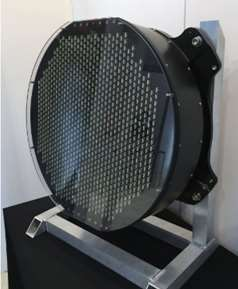
\includegraphics[width=\textwidth,height=3.5cm]{figs/aesa-antenna.png}
~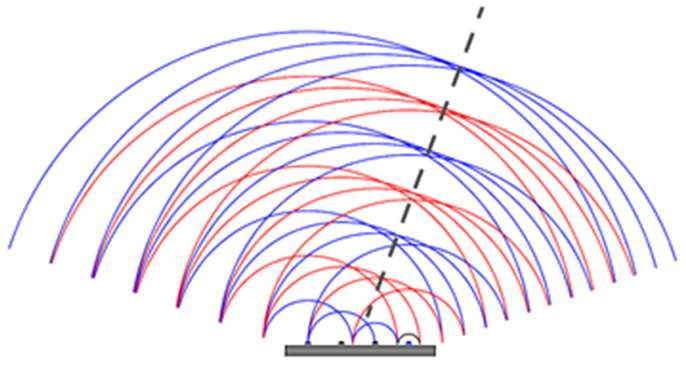
\includegraphics[width=\textwidth,height=3.5cm]{figs/aesa-beamforming.png}

Figure~\ref{fig:video-chain-spec} shows a simplified radar signal
processing chain that is used to illustrate the calculations of
interest. The input data from the antenna is processed in a number of
steps.

\begin{figure}
\hypertarget{fig:video-chain-spec}{%
\centering
\includegraphics{figs/video-chain-spec.pdf}
\caption{Overview of the video processing
chain}\label{fig:video-chain-spec}
}
\end{figure}

In this report we assume one stream per antenna element. The indata is
organized into a sequence of ``cubes'', each corresponding to a certain
integration interval. Each sample in the cube represents a particular
antenna element, pulse and range bin. The data of the cube arrives pulse
by pulse and each pulse arrives range bin by range bin. This is for all
elements in parallel. Between the Pulse Compression (PC) and Doppler
Filter Bank (DFB) steps there is a corner turn of data, i.e.~data from
all pulses must be collected before the DFB can execute.

The different steps of the chain, the antenna and the input data format
are briefly described in the following list. For a more detailed
description of the processing chain, please refer to
sections~\ref{sec:shallow}, \ref{sec:atom} respectively.

\begin{itemize}
\item
  \emph{Digital Beam Forming (DBF)}: The DBF step creates a number of
  simultaneous receiver beams, or ``listening directions'', from the
  input data. This is done by doing weighted combinations of the data
  from the different antenna elements, so that constructive interference
  is created in the desired bearings of the beams. The element samples
  in the input data set are then transformed into beams.
\item
  \emph{Pulse Compression (PC)}: The goal of the pulse compression is to
  collect all received energy from one target into a single range bin.
  The received echo of the modulated pulse is passed through a matched
  filter. Here, the matched filtering is done digitally.
\item
  \emph{Doppler Filter Bank incl.~envelope detection (DFB)}: The DFB
  gives an estimation of the target's speed relative to the radar. It
  also gives an improved signal-to-noise ratio due to a coherent
  integration of indata. The pulse bins in the data set are transformed
  into Doppler channels. The envelope detector calculates the absolute
  values of the digital samples. The data is real after this step.
\item
  \emph{Constant False Alarm Ratio (CFAR)}: The CFAR processing is
  intended to keep the number of false targets at an acceptable level
  while maintaining the best possible sensitivity. It normalizes the
  video in order to maintain a constant false alarm rate when the video
  is compared to a detection threshold. With this normalization the
  sensitivity will be adapted to the clutter situation in the area
  (around a cell under test) of interest.
\item
  \emph{Integrator (INT)} The integrator is an 8-tap unsigned integrator
  that integrates channel oriented video. Integration shall be done over
  a number of FFT batches of envelope detected video. Each Doppler
  channel, range bin and antenna element shall be integrated.
\end{itemize}

\hypertarget{sec:usage}{%
\subsection{Using This Document}\label{sec:usage}}

\textbf{PREREQUISITES:} the document assumes that the reader is familiar
with the functional programming language
\href{https://www.haskell.org/}{Haskell}, its syntax, and the usage of a
Haskell interpreter
(e.g.~\href{https://downloads.haskell.org/~ghc/latest/docs/html/users_guide/ghci.html}{\texttt{ghci}}).
Otherwise, we recommend consulting at least the introductory chapters of
one of the following books by Lipovača
(\protect\hyperlink{ref-Lipovaca11}{2011}) and Hutton
(\protect\hyperlink{ref-hutton-2016}{2016}) or other recent books in
Haskell. The reader also needs to be familiar with some basic ForSyDe
modeling concepts, such as \emph{process constructor}, \emph{process} or
\emph{signal}. We recommend going through at least the online getting
started
\href{https://forsyde.github.io/forsyde-shallow/getting_started}{tutorial
on ForSyDe-Shallow} or the one
\href{https://forsyde.github.io/forsyde-atom/assets/manual.pdf}{on
ForSyDe-Atom}, and if possible, consulting the (slightly outdated) book
chapter on ForSyDe ({\textbf{???}}).

This document has been created using literate programming. This means
that all code shown in the listings is compilable and executable. There
are two types of code listing found in this document. This style

\begin{Shaded}
\begin{Highlighting}[numbers=left,,]
\CommentTok{-- | API documentation comment}
\OtherTok{myIdFunc ::}\NormalTok{ a }\OtherTok{->}\NormalTok{ a}
\NormalTok{myIdFunc }\FunctionTok{=} \FunctionTok{id}
\end{Highlighting}
\end{Shaded}

shows \emph{source code} as it is found in the implementation files,
where the line numbers correspond to the position in the source file.
This style

\begin{verbatim}
Prelude> 1 + 1
2
\end{verbatim}

suggests \emph{interactive commands} given by the user in a terminal or
an interpreter session. The listing above shows a typical \texttt{ghci}
session, where the string after the prompter symbol
\texttt{\textgreater{}} suggests the user input (e.g.~\texttt{1\ +\ 1}).
Whenever relevant, the expected output is printed one row below
(e.g.~\texttt{2}).

The way this document is meant to be parsed efficiently is to load the
source files themselves in an interpreter and test the exported
functions gradually, while reading the document at the same time. Due to
multiple (sometimes conflicting) dependencies on external packages, for
convenience the source files are shipped as \emph{multiple}
\href{https://docs.haskellstack.org/en/stable/README/}{Stack} packages
each creating an own sandbox on the user's local machine with all
dependencies and requirements taken care of. Please refer to the
project's \texttt{README} file for instructions on how to install and
compile or run the Haskell files.

At the beginning of each chapter there is metadata guiding the reader
what tools and packages are used, like:

\begin{longtable}[]{@{}lll@{}}
\toprule
\endhead
Package & aesa-atom-0.1.0 & path:
\texttt{./aesa-atom/README.md}\tabularnewline
\bottomrule
\end{longtable}

This table tells that the package where the current chapter's code
resides is \texttt{aesa-atom}, version 0.1.0. This table might contain
information on the main dependency packages which contain important
functions, and which should be consulted while reading the code in the
current chapter. If the main package generates an executable binary or a
test suite, these are also pointed out. The third column provides
additional information such as a pointer to documentation (relative path
to the project root, or web URL), or usage suggestions.

It is recommended to read the main package's \texttt{README} file which
contains instructions on how to install, compile and test the software,
before proceeding with following a chapter. Each section of a chapter is
written within a library \emph{module}, pointed out in the beginning of
the respective section by the line:

\begin{Shaded}
\begin{Highlighting}[numbers=left,,]
\KeywordTok{module} \DataTypeTok{ForSyDe.X.Y} \KeywordTok{where}
\end{Highlighting}
\end{Shaded}

The most convenient way to test out all functions used in module
\texttt{ForSyDe.X.Y} is by loading its source file in the sandboxed
interpreter, i.e.~by running the following command from the project
root:

\begin{verbatim}
stack ghci src/ForSyDe/X/Y.lhs
\end{verbatim}

An equally convenient way is to create an own \texttt{.hs} file
somewhere under the project root, which imports and uses module
\texttt{ForSyDe.X.Y}, e.g.

\begin{Shaded}
\begin{Highlighting}[numbers=left,,]
\CommentTok{-- MyTest.hs}
\KeywordTok{import} \DataTypeTok{ForSyDe.X.Y}

\NormalTok{myData }\FunctionTok{=}\NormalTok{ [}\DecValTok{1}\NormalTok{,}\DecValTok{2}\NormalTok{,}\DecValTok{3}\NormalTok{,}\DecValTok{4}\NormalTok{,}\DecValTok{5}\NormalTok{]}\OtherTok{ ::}\NormalTok{ [}\DataTypeTok{Int}\NormalTok{]}
\NormalTok{myTest }\FunctionTok{=}\NormalTok{ functionFromForSyDeXY myData}
\end{Highlighting}
\end{Shaded}

This file can be loaded and/or compiled from within the sandbox,
e.g.~with \texttt{stack\ ghci\ MyTest.hs}.

\clearpage

\hypertarget{sec:atom}{%
\section{High-Level Model of the AESA Signal Processing Chain in
ForSyDe-Atom}\label{sec:atom}}

\begin{quote}
\emph{This section guides the reader throughout converting the provided
specifications of the AESA signal processing chain into a concrete,
functionally complete, high-level executable model in ForSyDe-Atom.
Enough AESA system details are given in order to understand the modeling
decisions. At the end of this section we simulate this model against a
realistic input set of complex antenna data, and test if it is sane
(i.e.~provides the expected results).}
\end{quote}

\begin{longtable}[]{@{}lll@{}}
\toprule
\endhead
Package & aesa-atom-0.1.0 & path:
\texttt{./aesa-atom/README.md}\tabularnewline
Deps & forsyde-atom-0.2.2 & url:
\texttt{https://forsyde.github.io/forsyde-atom/api/}\tabularnewline
& forsyde-atom-extensions-0.1.1 & path:
\texttt{./forsyde-atom-extensions/README.md}\tabularnewline
Bin & aesa-hl & usage: \texttt{aesa-hl\ -\/-help}\tabularnewline
\bottomrule
\end{longtable}

Historically,
\href{https://forsyde.github.io/forsyde-atom/}{ForSyDe-Atom} has been a
spin-off of
\href{https://forsyde.github.io/forsyde-shallow/}{ForSyDe-Shallow} which
has explored new modeling concepts, and had a fundamentally different
approach to how models are described and instantiated. ForSyDe-Atom
introduced the concept of \emph{language layer}, extending the idea of
process constructor, and within this setting it explored the algebra of
algorithmic skeletons, employed heavily within this report. As of today,
both ForSyDe-Shallow and ForSyDe-Atom have similar APIs and are capable
of modeling largely the same behaviors. The main syntax differences
between the two are covered in section~\ref{sec:shallow}, where the same
high-level model is written in ForSyDe-Shallow.

\hypertarget{sec:crash-atom}{%
\subsection{Crash course in ForSyDe-Atom}\label{sec:crash-atom}}

Before proceeding with the modeling of the AESA processing chain, let us
consolidate the main ForSyDe concepts which will be used throughout this
report: \emph{layer}, \emph{process constructor} and \emph{skeleton}. If
you are not familiar with ForSyDe nomenclature and general modeling
principles, we recommend consulting the documentation pointed out in
section~\ref{sec:intro} first.

As seen in section~\ref{sec:video-chain-spec}, most of the AESA
application consists of typical DSP algorithms such as matrix
multiplications, FFT, moving averages, etc. which lend themselves to
\emph{streaming parallel} implementations. Hence we need to
unambiguously capture the two distinct aspects of the AESA chain
components:

\begin{itemize}
\item
  \emph{streaming behavior} is expressed in ForSyDe through processes
  which operate on signals encoding a temporal partitioning of data.
  Processes are instantiated exclusively using \emph{process
  constructors} which can be regarded as templates inferring the
  semantics of computation, synchronization and concurrency as dictated
  by a certain model of computation (MoC) (Sander and Jantsch
  (\protect\hyperlink{ref-sander-2004}{2004}),Lee and Seshia
  (\protect\hyperlink{ref-leeseshia-15}{2016})).
\item
  \emph{parallelism} is expressed through parallel patterns which
  operate on structured types (e.g.~vectors) encoding a spatial
  partitioning of data. These patterns are instantiated as skeletons,
  which are templates inferring the semantics of distribution, parallel
  computation and interaction between elements, as defined by the
  algebra of catamorphisms (Fischer, Gorlatch, and Bischof
  \protect\hyperlink{ref-Fischer-2003}{2003}).
\end{itemize}

\begin{figure}
\hypertarget{fig:atom-layers}{%
\centering
\includegraphics{figs/layers.pdf}
\caption{Depiction of layer usage: (left) skeleton networks of
processes; (right) processes of skeleton
functions}\label{fig:atom-layers}
}
\end{figure}

In order to capture these two\footnote{and other aspects, not covered in
  this report} interacting aspects in unison as a complete system, we
describe them in terms of two distinct, orthogonal \emph{layers} within
the ForSyDe-Atom framework. A language layer is a (very small) domain
specific language (DSL) heavily rooted in the functional programming
paradigm, which is able to describe one aspect of a cyber-physical
system (CPS). Layers interact with one another by virtue of the
abstraction principle inherent to a functional programming language
(Backus \protect\hyperlink{ref-backus-1978}{1978}): each layer defines
at least one higher order function that is able to take a function
(i.e.~abstraction) from another layer as an argument and to lift it
within its own domain. To nepicture the interaction between layers,
consider Figure~\ref{fig:video-chain-spec} where, although we use the
same \texttt{farm} vector skeleton and \texttt{comb} synchronous (SY)
process constructor, the two different compositions describe two
different (albeit semantically equivalent) systems: the first one is
instantiating a farm network of SY processes operating on a vector of
signals in parallel; whereas the second one is instantiating a single SY
process operating on o signal where each event is carrying a vector of
values.

\hypertarget{sec:atom-network}{%
\subsection{The High-Level Model}\label{sec:atom-network}}

This section presents a high-level behavioral model of the AESA signal
processing chain presented in section~\ref{sec:video-chain-spec}, which
is, in any circumstance, \emph{not} the only modeling alternative, but
rather shows an intuitive and didactic way to tackle the challenge of
translating the \emph{textual} specifications into an \emph{executable}
ForSyDe specification. While most design choices are driven by the
ambition to introduce the new modeling concepts presented in
section~\ref{sec:crash-atom}, they can be justified by the need to
capture the essential behavioral properties in a formal way, in order to
be exploitable in future stages of a design flow towards efficient
implementations. The main design approach is to exploit the relative
independence between each data path associated with each antenna element
or beam, and to model these paths as skeletons (e.g.~farms) of (chains
of) processes. Each design decision will infer a re-partitioning of the
indata cubes between the time/causality and space dimensions following
the design patters depicted in Figure~\ref{fig:atom-layers}, namely:

\begin{itemize}
\item
  \emph{skeletons of processes} which: 1) express parallelism at the
  process level; 2) depicts processes as operating on elementary streams
  of data, e.g.~originating from each antenna element in particular, and
  skeletons as the structured interactions between these streams; 3)
  expose a fine-grained modular view allowing to quantify the potential
  for \emph{load distribution}, since each ``operation'' (i.e.~process)
  clearly captures the aspect of precedence constraints.
\item
  \emph{process of skeletons} which : 1) express parallelism at the
  datum level; 2) depicts processes as operating on structures of data
  (e.g.~vectors, matrices or cubes); 3) expose a monolithic view of
  processes where precedence constraints are expressed ``outside'' of
  the algorithm, and where the algorithm itself expresses potential for
  \emph{data parallelism}.
\end{itemize}

The code for this section is written in the following module, see
section~\ref{sec:usage} on how to use it:

\begin{Shaded}
\begin{Highlighting}[numbers=left,,firstnumber=33,]
\OtherTok{\{-# LANGUAGE PackageImports #-\}} \CommentTok{-- allows explicit import of modules from custom}
                                \CommentTok{-- libraries instead of standard ones. Will be taken}
                                \CommentTok{-- out once the extensions are merged upstream.}
\KeywordTok{module} \DataTypeTok{ForSyDe.AESA.HighLevelAtom} \KeywordTok{where}
\end{Highlighting}
\end{Shaded}

\hypertarget{imported-libraries}{%
\subsubsection{Imported Libraries}\label{imported-libraries}}

As the AESA application uses complex numbers, we use Haskell's
\href{http://hackage.haskell.org/package/base/docs/Data-Complex.html}{\texttt{Complex}}
type.

\begin{Shaded}
\begin{Highlighting}[numbers=left,,firstnumber=43,]
\KeywordTok{import} \DataTypeTok{Data.Complex}
\end{Highlighting}
\end{Shaded}

For describing streaming behavior of the application our design will use
a heterogeneous approach, using a combination of \emph{synchronous
reactive (SY)} processes (Lee and Seshia
(\protect\hyperlink{ref-leeseshia-15}{2016}),Benveniste et al.
(\protect\hyperlink{ref-Benveniste03}{2003})), where the main assumption
is that all events in the system are synchronized; and \emph{synchronous
data flow (SDF)} processes (Lee and Seshia
(\protect\hyperlink{ref-leeseshia-15}{2016}),Lee and Parks
(\protect\hyperlink{ref-lee95}{1995})), where the temporal behavior is
formulated in terms of partial order constraints between events. We
import the
\href{https://forsyde.github.io/forsyde-atom/api/ForSyDe-Atom-MoC-SY.html}{\texttt{SY}}
and
\href{https://forsyde.github.io/forsyde-atom/api/ForSyDe-Atom-MoC-SDF.html}{\texttt{SDF}}
libraries described in the
\emph{\href{https://forsyde.github.io/forsyde-atom/api/ForSyDe-Atom-MoC.html}{MoC}
layer}, see (Ungureanu and Sander
\protect\hyperlink{ref-ungureanu17}{2017}), using an appropriate alias
for each.

\begin{Shaded}
\begin{Highlighting}[numbers=left,,firstnumber=57,]
\KeywordTok{import}\NormalTok{ "forsyde-atom-extensions" }\DataTypeTok{ForSyDe.Atom.MoC.SY}  \KeywordTok{as} \DataTypeTok{SY}
\KeywordTok{import}\NormalTok{ "forsyde-atom-extensions" }\DataTypeTok{ForSyDe.Atom.MoC.SDF} \KeywordTok{as} \DataTypeTok{SDF}
\end{Highlighting}
\end{Shaded}

For describing parallel operations on data we use algorithmic skeletons
(Fischer, Gorlatch, and Bischof
(\protect\hyperlink{ref-Fischer-2003}{2003}),Skillicorn
(\protect\hyperlink{ref-skillicorn05}{2005})), formulated on
ForSyDe-Atom's in-house
\href{http://hackage.haskell.org/package/forsyde-shallow/docs/ForSyDe-Shallow-Core-Vector.html}{\texttt{Vector}}
data type, which is a shallow, lazy-evaluated implementation of
unbounded arrays, ideal for early design validation. Although dependent,
bounded, and even boxed (i.e.~memory-mapped) alternatives exist, such as
\href{http://hackage.haskell.org/package/parameterized-data/docs/Data-Param-FSVec.html}{\texttt{FSVec}}
or REPA \href{http://hackage.haskell.org/package/repa}{\texttt{Array}}s,
for the scope of this project the functional validation and (by-hand)
requirement analysis on the properties of skeletons will suffice. We
also import the \texttt{Matrix} and \texttt{Cube} utility libraries
which contain type synonyms for nested \texttt{Vector}s along with their
derived skeletons, as well a \texttt{DSP} which contain commonly used
DSP blocks defined in terms of vector skeletons.

\begin{Shaded}
\begin{Highlighting}[numbers=left,,firstnumber=74,]
\KeywordTok{import}\NormalTok{ "forsyde-atom-extensions" }\DataTypeTok{ForSyDe.Atom.Skeleton.Vector}        \KeywordTok{as} \DataTypeTok{V}
\KeywordTok{import}\NormalTok{ "forsyde-atom-extensions" }\DataTypeTok{ForSyDe.Atom.Skeleton.Vector.Cube}   \KeywordTok{as} \DataTypeTok{C}
\KeywordTok{import}\NormalTok{ "forsyde-atom-extensions" }\DataTypeTok{ForSyDe.Atom.Skeleton.Vector.Matrix} \KeywordTok{as} \DataTypeTok{M}
\KeywordTok{import}\NormalTok{ "forsyde-atom-extensions" }\DataTypeTok{ForSyDe.Atom.Skeleton.Vector.DSP}
\end{Highlighting}
\end{Shaded}

\hypertarget{sec:aliases-shallow}{%
\subsubsection{Type Aliases and Constants}\label{sec:aliases-shallow}}

For ease of documentation we will be using type synonyms (aliases) for
all types and structures throughout this design:

\begin{itemize}
\item
  \texttt{Antenna} denotes a vector container for the antenna elements.
  Its length is equal to the number of antennas in the radar \(N_A\).
\item
  After Digital Beamforming (DBF), the antenna elements are transformed
  into \(N_B\) beams, thus we associate the \texttt{Beam} alias for the
  vector container wrapping those beams.
\item
  \texttt{Range} is a vector container for range bins. All antennas have
  the same number of range bins \(N_b\), rendering each
  \(\text{Antenna} \times \text{Range}\) a perfect matrix of samples for
  every pulse.
\item
  \texttt{Window} stands for a Doppler window of \(N_{FFT}\) pulses.
\end{itemize}

\begin{Shaded}
\begin{Highlighting}[numbers=left,,firstnumber=97,]
\KeywordTok{type} \DataTypeTok{Antenna}     \FunctionTok{=} \DataTypeTok{Vector} \CommentTok{-- length: nA}
\KeywordTok{type} \DataTypeTok{Beam}        \FunctionTok{=} \DataTypeTok{Vector} \CommentTok{-- length: nB}
\KeywordTok{type} \DataTypeTok{Range}       \FunctionTok{=} \DataTypeTok{Vector} \CommentTok{-- length: nb}
\KeywordTok{type} \DataTypeTok{Window}      \FunctionTok{=} \DataTypeTok{Vector} \CommentTok{-- length: nFFT}
\end{Highlighting}
\end{Shaded}

Here we define the size constants, for a simple test scenario provided
by Saab AB. The size \texttt{nA} can be inferred from the size of input
data and the vector operations.

\begin{Shaded}
\begin{Highlighting}[numbers=left,,firstnumber=105,]
\NormalTok{nA   }\FunctionTok{=}   \DecValTok{16}\OtherTok{ ::} \DataTypeTok{Int} \CommentTok{-- does not really affect the application}
\NormalTok{nB   }\FunctionTok{=}    \DecValTok{8}\OtherTok{ ::} \DataTypeTok{Int}
\NormalTok{nb   }\FunctionTok{=} \DecValTok{1024}\OtherTok{ ::} \DataTypeTok{Int}
\NormalTok{nFFT }\FunctionTok{=}  \DecValTok{256}\OtherTok{ ::} \DataTypeTok{Int}
\end{Highlighting}
\end{Shaded}

Finally we provide two aliases for the basic Haskell data types used in
the system, to stay consistent with the application specification.

\begin{Shaded}
\begin{Highlighting}[numbers=left,,firstnumber=113,]
\KeywordTok{type} \DataTypeTok{CpxData}  \FunctionTok{=} \DataTypeTok{Complex} \DataTypeTok{Float}
\KeywordTok{type} \DataTypeTok{RealData} \FunctionTok{=} \DataTypeTok{Float}
\end{Highlighting}
\end{Shaded}

\hypertarget{video-processing-stages}{%
\subsubsection{Video Processing Stages}\label{video-processing-stages}}

In this section we follow each stage described in
section~\ref{sec:video-chain-spec}, and exploit the initial assumption
on the order of events stating: \emph{``For each antenna the data
arrives \emph{pulse by pulse}, and each pulse arrives \emph{range bin by
range bin}. This happens \emph{for all antennas in parallel}, and all
complex samples are synchronized with the same sampling rate, e.g.~of
the A/D converter.''}

This allows us to ``unroll'' the indata video cubes into \(N_A\)
parallel synchronous streams, each stream being able to be processed as
soon as it contains enough data. This unrolling is depicted in
Figure~\ref{fig:cube-unrolling} as streaming the pulses as soon as they
arrive: range bin by range bin. We say that we partition the data
\emph{in time} rather than \emph{in space}, which is a more appropriate
partition judging by the assumption above.

\begin{figure}
\hypertarget{fig:cube-unrolling}{%
\centering
\includegraphics{figs/cube-unrolling.pdf}
\caption{Video cube unrolling}\label{fig:cube-unrolling}
}
\end{figure}

\hypertarget{sec:dbf-atom-net}{%
\paragraph{Digital Beamforming (DBF)}\label{sec:dbf-atom-net}}

The DBF receives complex in data, from \(N_A\) antenna elements and
forms \(N_B\) simultaneous receiver beams, or ``listening directions'',
by summing individually phase-shifted in data signals from all elements.
Depicted from a streaming point of view, DBF would like in
Figure~\ref{fig:dbf-samp}.

\begin{figure}
\hypertarget{fig:dbf-samp}{%
\centering
\includegraphics{figs/dbf-samp.pdf}
\caption{Digital Beam Forming on streams of complex
samples}\label{fig:dbf-samp}
}
\end{figure}

As can be seen in Figure~\ref{fig:dbf-samp}, a beam can be formed
\emph{as soon as} all antennas have produced a complex sample. The
parallel streams of data coming from each antenna element are
represented as a \emph{vector of synchronous (SY) signals}, i.e.~vector
of signals where each event is synchronous with each other. This allows
us to depict the dataflow interaction between the streams during digital
beamforming as the process network in Figure~\ref{fig:dbf-net-atom},
where an \(\oplus\) represents a combinational process
\href{https://forsyde.github.io/forsyde-atom/api/ForSyDe-Atom-MoC.html\#v:comb22}{\texttt{comb}}.

\begin{figure}
\hypertarget{fig:dbf-net-atom}{%
\centering
\includegraphics{figs/dbf-net-atom.pdf}
\caption{DBF network}\label{fig:dbf-net-atom}
}
\end{figure}

\begin{Shaded}
\begin{Highlighting}[numbers=left,,firstnumber=153,]
\OtherTok{dbf ::} \DataTypeTok{Antenna}\NormalTok{ (}\DataTypeTok{SY.Signal} \DataTypeTok{CpxData}\NormalTok{)}
    \OtherTok{->} \DataTypeTok{Beam}\NormalTok{    (}\DataTypeTok{SY.Signal} \DataTypeTok{CpxData}\NormalTok{)}
\NormalTok{dbf antennaSigs }\FunctionTok{=}\NormalTok{ beamSigs}
  \KeywordTok{where}
\NormalTok{    beamSigs   }\FunctionTok{=}\NormalTok{ V.farm11 (V.reduce (SY.comb21 (}\FunctionTok{+}\NormalTok{))) beamMatrix}
\NormalTok{    beamMatrix }\FunctionTok{=}\NormalTok{ M.farm21 (\textbackslash{}c }\OtherTok{->}\NormalTok{ SY.comb11 (}\FunctionTok{*}\NormalTok{c)) beamConsts sigMatrix}
\NormalTok{    sigMatrix  }\FunctionTok{=}\NormalTok{ V.farm11 V.fanout antennaSigs}
\NormalTok{    beamConsts }\FunctionTok{=}\NormalTok{ mkBeamConsts (V.length antennaSigs) nB}
\end{Highlighting}
\end{Shaded}

\begin{longtable}[]{@{}lll@{}}
\toprule
Function & Original module & Package\tabularnewline
\midrule
\endhead
\texttt{farm11}, \texttt{reduce}, \texttt{length} &
\href{https://forsyde.github.io/forsyde-atom/api/ForSyDe-Atom-Skeleton-Vector.html}{\texttt{ForSyDe.Atom.Skeleton.Vector}}
& forsyde-atom\tabularnewline
\texttt{farm21} & \texttt{ForSyDe.Atom.Skeleton.Vector.Matrix} &
forsyde-atom-extensions\tabularnewline
\texttt{comb11}, \texttt{comb21} &
\href{https://forsyde.github.io/forsyde-atom/api/ForSyDe-Atom-MoC-SY.html}{\texttt{ForSyDe.Atom.MoC.SY}}
& forsyde-atom\tabularnewline
\texttt{mkBeamConsts} & \texttt{ForSyDe.AESA.Coefs} &
aesa-atom\tabularnewline
\bottomrule
\end{longtable}

The previous code listing, depicted in Figure~\ref{fig:dbf-net-atom}, is
actually showing the ``internals'' of a matrix-vector dot
product\footnote{see \texttt{dotMatMat} in the
  \texttt{ForSyDe.Atom.Skeleton.Vector.DSP} module from package
  \texttt{forsyde-atom-extensions}.}. However, the elementary
operations, instead of regular arithmetic operations \(\times\) and
\(+\), are \emph{processes} applying these operations on SY streams. As
such, the \texttt{fanout} skeleton distributes one signal to a whole row
(i.e.~vector) of processes, the matrix \texttt{farm} applies pair-wise a
matrix of partially applied processes on this matrix of signals, and
\texttt{reduce} creates a reduction network of binary processes
pair-wise applying the function \(+\) on all events in signals.
Practically the DBF network transforms \(N_A\) synchronous signals
originating from each antenna element into \(N_B\) synchronous signals
for each beam. The internal structure of this transformation exposes
multiple degrees of potential distribution on parallel synchronous
resources.

The table above gives some pointers where to look for additional
documentation of each imported function. The formula to generate the
beam constants \texttt{mkBeamConsts} is presented later in
section~\ref{sec:atom-coefs}.

\hypertarget{sec:pc-atom-net}{%
\paragraph{Pulse Compression (PC)}\label{sec:pc-atom-net}}

In this stage the received echo of the modulated pulse, i.e.~the
information contained by the range bins, is passed through a matched
filter for decoding their modulation. This essentially applies a sliding
window, or a moving average (MAV) on the range bin samples.

\begin{figure}
\hypertarget{fig:pc-samp}{%
\centering
\includegraphics{figs/pc-samp.pdf}
\caption{Pulse Compression on streams of complex
samples}\label{fig:pc-samp}
}
\end{figure}

In Figure~\ref{fig:pc-samp} we can see that, in order to apply the MAV
algorithm on all the range bins of every pulse, we need to accumulate
\(N_b\) samples and process them in batches. Intuitively this can be
done by processing each beam with a \emph{synchronous dataflow} (SDF)
actor which, with each firing, consumes \(N_b\) samples and produces
\(N_b\) samples. Note that at this stage of modeling we value intuition
and the capturing of the right application properties rather than
efficiency. We will tackle this problem later in the design stages (see
section~\ref{sec:refinement}) where we will try to transform the model
toward more ``efficient'' implementation models (with respect to some
constraint, e.g.~throughput) which preserve these behavioral properties.

\begin{figure}
\hypertarget{fig:pc-proc-atom}{%
\centering
\includegraphics{figs/pc-proc-atom.pdf}
\caption{PC stage process}\label{fig:pc-proc-atom}
}
\end{figure}

\begin{Shaded}
\begin{Highlighting}[numbers=left,,firstnumber=210,]
\OtherTok{pc ::} \DataTypeTok{Beam}\NormalTok{ ( }\DataTypeTok{SY.Signal} \DataTypeTok{CpxData}\NormalTok{)}
   \OtherTok{->} \DataTypeTok{Beam}\NormalTok{ (}\DataTypeTok{SDF.Signal} \DataTypeTok{CpxData}\NormalTok{)}
\NormalTok{pc }\FunctionTok{=}\NormalTok{ V.farm11 (procPC }\FunctionTok{.}\NormalTok{ SY.toSDF)}
\end{Highlighting}
\end{Shaded}

\begin{longtable}[]{@{}lll@{}}
\toprule
Function & Original module & Package\tabularnewline
\midrule
\endhead
\texttt{farm11} &
\href{https://forsyde.github.io/forsyde-atom/api/ForSyDe-Atom-Skeleton-Vector.html}{\texttt{ForSyDe.Atom.Skeleton.Vector}}
& forsyde-atom\tabularnewline
\texttt{toSDF} &
\href{https://forsyde.github.io/forsyde-atom/api/ForSyDe-Atom-MoC-SY.html}{\texttt{ForSyDe.Atom.MoC.SY}}
& forsyde-atom\tabularnewline
\texttt{comb11} &
\href{https://forsyde.github.io/forsyde-atom/api/ForSyDe-Atom-MoC-SDF.html}{\texttt{ForSyDe.Atom.MoC.SDF}}
& forsyde-atom\tabularnewline
\texttt{mav} & \texttt{ForSyDe.Atom.Skeleton.Vector.DSP} &
forsyde-atom-extensions\tabularnewline
\texttt{mkPcCoefs} & \texttt{ForSyDe.AESA.Coefs} &
aesa-atom\tabularnewline
\bottomrule
\end{longtable}

Following the reasoning above, we instantiate the PC video processing
stage as a \texttt{farm} of SDF processes \texttt{procPC} as depicted in
Figure~\ref{fig:pc-proc-atom}. Notice that before being able to apply
the SDF actors we need to translate the SY signals yielded by the DBF
stage into SDF signals. This is done by the \texttt{toSDF} interface
which is an injective mapping from the (timed) domain of a SY MoC tag
system, to the (untimed) codomain of a SDF MoC tag system. For more on
tag systems please consult (Lee and Sangiovanni-Vincentelli
\protect\hyperlink{ref-lee98}{1998}).

\begin{Shaded}
\begin{Highlighting}[numbers=left,,firstnumber=229,]
\OtherTok{procPC ::} \DataTypeTok{Fractional}\NormalTok{ a }\OtherTok{=>} \DataTypeTok{SDF.Signal}\NormalTok{ a }\OtherTok{->} \DataTypeTok{SDF.Signal}\NormalTok{ a }
\NormalTok{procPC }\FunctionTok{=}\NormalTok{ SDF.comb11 (nb, nb, V.fromVector }\FunctionTok{.}\NormalTok{ mav mkPcCoefs }\FunctionTok{.}\NormalTok{ V.vector)}
\end{Highlighting}
\end{Shaded}

The \texttt{procPC} actor consumes and produces \texttt{nb} tokens each
firing, forms a \texttt{Vector} from these tokens, and applies the
\texttt{mav} skeleton on these vectors. The \texttt{mav} skeleton is a
utility formulated in terms of primitive skeletons (i.e.~\texttt{map}
and \texttt{reduce}) on numbers, i.e.~lifting arithmetic functions. We
will study this skeleton later in this report and for now we take it
``for granted'', as conveniently provided by the \texttt{DSP} utility
library. Also notice that the type signature for \texttt{procPC} is left
polymorphic as to be more convenient later when we formulate properties
over it.

\hypertarget{corner-turn-ct}{%
\paragraph{Corner Turn (CT)}\label{corner-turn-ct}}

In order to be able to calculate the Doppler channels further in the
processing pipeline, during a CT, a rearrangement of data must be
performed between functions that process data in ``different''
directions, e.g.~range and pulse. This rearrangement is called corner
turn. We make use of the knowledge that for each beam samples arrive in
order, one range bin at a time, in the direction of consumption
suggested in Figure~\ref{fig:ct-samp}, and ``fill back in'' the video
cube in the direction of production. In order to maximize the efficiency
of the AESA processing the datapath is split into two concurrent
processing channels with 50\% overlapped data, as depicted in
Figure~\ref{fig:ct-cube}.

\begin{figure}
\hypertarget{fig:ct-samp}{%
\centering
\includegraphics{figs/ct-samp.pdf}
\caption{Building matrices of complex samples during
CT}\label{fig:ct-samp}
}
\end{figure}

\begin{figure}
\hypertarget{fig:ct-cube}{%
\centering
\includegraphics{figs/ct-cube.pdf}
\caption{Concurrent processing on 50\% overlapped
data}\label{fig:ct-cube}
}
\end{figure}

Our CT network thus maps on each beam signal a corner turn process
which, under the SDF execution semantics, consumes \(N_{FFT}\times N_b\)
(ordered) samples, interprets it as a matrix, transposes it, and
produces \(N_b\times N_{FFT}\) samples ordered in the direction
suggested in Figure~\ref{fig:ct-samp}. In order to achieve 50\%
overlapping between the two output channels, the left one needs to be
``delayed'' with a prefix signal equivalent to half a video cube. In
this case that prefix is formed of \(\frac{N_b \times N_{FFT}}{2}\)
complex zeroes on each beam path. This way, whatever input arrives from
the PC stage, will be observed at the left channel only after
\(N_{FFT}/2\) samples.

\begin{figure}
\hypertarget{fig:ct-net-atom}{%
\centering
\includegraphics{figs/ct-net-atom.pdf}
\caption{CT network}\label{fig:ct-net-atom}
}
\end{figure}

\begin{Shaded}
\begin{Highlighting}[numbers=left,,firstnumber=269,]
\OtherTok{ct ::} \DataTypeTok{Beam}\NormalTok{ (}\DataTypeTok{SDF.Signal} \DataTypeTok{CpxData}\NormalTok{)}
   \OtherTok{->}\NormalTok{ (}\DataTypeTok{Beam}\NormalTok{ (}\DataTypeTok{SDF.Signal} \DataTypeTok{CpxData}\NormalTok{),}
       \DataTypeTok{Beam}\NormalTok{ (}\DataTypeTok{SDF.Signal} \DataTypeTok{CpxData}\NormalTok{))}
\NormalTok{ct }\FunctionTok{=}\NormalTok{ V.farm12 procCT}

\OtherTok{procCT ::} \DataTypeTok{Num}\NormalTok{ a }\OtherTok{=>} \DataTypeTok{SDF.Signal}\NormalTok{ a }\OtherTok{->}\NormalTok{ (}\DataTypeTok{SDF.Signal}\NormalTok{ a, }\DataTypeTok{SDF.Signal}\NormalTok{ a)}
\NormalTok{procCT sig }\FunctionTok{=}\NormalTok{ (rightChannel, leftChannel)}
  \KeywordTok{where}
\NormalTok{    rightChannel }\FunctionTok{=}\NormalTok{ cornerTurn sig}
\NormalTok{    leftChannel  }\FunctionTok{=}\NormalTok{ SDF.delay initBatch rightChannel}
\NormalTok{    initBatch    }\FunctionTok{=} \FunctionTok{replicate}\NormalTok{ (nb }\FunctionTok{*}\NormalTok{ nFFT }\OtherTok{`div`} \DecValTok{2}\NormalTok{) }\DecValTok{0}
\NormalTok{    cornerTurn   }\FunctionTok{=}\NormalTok{ SDF.comb11 (nFFT }\FunctionTok{*}\NormalTok{ nb, nb }\FunctionTok{*}\NormalTok{ nFFT,}
\NormalTok{                               fromMatrix }\FunctionTok{.}\NormalTok{ M.transpose }\FunctionTok{.}\NormalTok{ matrix nb nFFT)}
\end{Highlighting}
\end{Shaded}

\begin{longtable}[]{@{}lll@{}}
\toprule
\begin{minipage}[b]{0.30\columnwidth}\raggedright
Function\strut
\end{minipage} & \begin{minipage}[b]{0.37\columnwidth}\raggedright
Original module\strut
\end{minipage} & \begin{minipage}[b]{0.24\columnwidth}\raggedright
Package\strut
\end{minipage}\tabularnewline
\midrule
\endhead
\begin{minipage}[t]{0.30\columnwidth}\raggedright
\texttt{farm12}\strut
\end{minipage} & \begin{minipage}[t]{0.37\columnwidth}\raggedright
\href{https://forsyde.github.io/forsyde-atom/api/ForSyDe-Atom-Skeleton-Vector.html}{\texttt{ForSyDe.Atom.Skeleton.Vector}}\strut
\end{minipage} & \begin{minipage}[t]{0.24\columnwidth}\raggedright
forsyde-atom\strut
\end{minipage}\tabularnewline
\begin{minipage}[t]{0.30\columnwidth}\raggedright
(\texttt{from}-)\texttt{matrix}, \texttt{transpose}\strut
\end{minipage} & \begin{minipage}[t]{0.37\columnwidth}\raggedright
\texttt{ForSyDe.Atom.Skeleton.Vector.Matrix}\strut
\end{minipage} & \begin{minipage}[t]{0.24\columnwidth}\raggedright
forsyde-atom-extensions\strut
\end{minipage}\tabularnewline
\begin{minipage}[t]{0.30\columnwidth}\raggedright
\texttt{comb11}, \texttt{delay}\strut
\end{minipage} & \begin{minipage}[t]{0.37\columnwidth}\raggedright
\href{https://forsyde.github.io/forsyde-atom/api/ForSyDe-Atom-MoC-SDF.html}{\texttt{ForSyDe.Atom.MoC.SDF}}\strut
\end{minipage} & \begin{minipage}[t]{0.24\columnwidth}\raggedright
forsyde-atom\strut
\end{minipage}\tabularnewline
\bottomrule
\end{longtable}

\emph{Interesting fact:} although the application specification mentions
that the first \(N_{FFT}\) batch of pulses is ignored, we cannot do that
at this stage. In fact ForSyDe does not allow ``cleaning up''
(i.e.~dropping, ignoring) events from signals, due to non-determinism
introduced in case of possible feedback loops. Only an observer
(i.e.~testbench, sink) is allowed to do that, outside the process
network. Furthermore, due to Haskell's lazy evaluation, ignoring some
output values means that those values are not even computed to start
with.

\hypertarget{sec:dfb-atom-net}{%
\paragraph{Doppler Filter Bank (DFB)}\label{sec:dfb-atom-net}}

During the Doppler filter bank, every window of samples, associated with
each range bin goes through a transformation consisting in weighting,
FFT, and envelope calculation, as already presented in
section~\ref{sec:dfb-shallow}. Since the samples have been arranged in
pulse window-order during the previous stage, the DFB transformation can
occur as soon as a window of \(N_{FFT}\) samples arrive, like in
Figure~\ref{fig:dfb-samp}.

\begin{figure}
\hypertarget{fig:dfb-samp}{%
\centering
\includegraphics{figs/dfb-samp.pdf}
\caption{Doppler Filter Bank on streams of complex
samples}\label{fig:dfb-samp}
}
\end{figure}

In contrast with the pulse compression (PC) stage in
section~\ref{sec:pc-atom-net}, the DFB is not carried out in a ``sliding
window'' fashion, i.e.~it cannot be processed ``one sample at a time'',
but rather it needs the whole \(N_{FFT}\) batch in order to apply the
FFT algorithm. As such, the best-fitted MoC execution semantics to
describe the process(es) associated with DFB is still SDF. We can simply
describe the DFB stage as a
\href{https://forsyde.github.io/forsyde-atom/api/ForSyDe-Atom-Skeleton-Vector.html\#v:farm22}{\texttt{farm}}
of
\href{https://forsyde.github.io/forsyde-atom/api/ForSyDe-Atom-MoC-SDF.html\#v:comb22}{\texttt{comb}}
SDF actors which apply the \(f_{DFB}\) function on \(N_{FFT}\) tokens
every firing cycle, as seen in Figure~\ref{fig:dfb-net-atom}.

\begin{figure}
\hypertarget{fig:dfb-net-atom}{%
\centering
\includegraphics{figs/dfb-net-atom.pdf}
\caption{DFB network}\label{fig:dfb-net-atom}
}
\end{figure}

\begin{Shaded}
\begin{Highlighting}[numbers=left,,firstnumber=325,]
\OtherTok{dfb ::} \DataTypeTok{Beam}\NormalTok{ (}\DataTypeTok{SDF.Signal} \DataTypeTok{CpxData}\NormalTok{)}
    \OtherTok{->} \DataTypeTok{Beam}\NormalTok{ (}\DataTypeTok{SDF.Signal} \DataTypeTok{RealData}\NormalTok{)}
\NormalTok{dfb }\FunctionTok{=}\NormalTok{ V.farm11}
\NormalTok{      (SDF.comb11 (nFFT, nFFT,}
\NormalTok{                   fromVector }\FunctionTok{.}\NormalTok{ fDFB }\FunctionTok{.}\NormalTok{ vector))}
  \KeywordTok{where}
\NormalTok{    fDFB       }\FunctionTok{=}\NormalTok{ V.farm11 envelope }\FunctionTok{.}\NormalTok{ fft nFFT }\FunctionTok{.}\NormalTok{ weight }
\NormalTok{    weight     }\FunctionTok{=}\NormalTok{ V.farm21 (}\FunctionTok{*}\NormalTok{) mkWeightCoefs}
\NormalTok{    envelope a }\FunctionTok{=} \KeywordTok{let}\NormalTok{ i }\FunctionTok{=}\NormalTok{ realPart a}
\NormalTok{                     q }\FunctionTok{=}\NormalTok{ imagPart a}
                 \KeywordTok{in} \FunctionTok{sqrt}\NormalTok{ (i }\FunctionTok{*}\NormalTok{ i }\FunctionTok{+}\NormalTok{ q }\FunctionTok{*}\NormalTok{ q)}
\end{Highlighting}
\end{Shaded}

Each function composing \(f_{DFB}\) is itself inherently parallel, as it
is described in terms of parallel skeletons. We could have ``lifted''
these skeletons as deep as associating a process for each elementary
arithmetic operation, following the example set in
section~\ref{sec:dbf-atom-net}. This, however, is left as an exercise
for the reader. The interested reader is also recommended to read the
associated chapter in the technical manual (Ungureanu
(\protect\hyperlink{ref-atom-manual}{2018})) to see how the
\texttt{fft\textquotesingle{}}\footnote{see
  \texttt{ForSyDe.Atom.Skeleton.Vector.DSP.fft\textquotesingle{}} from
  the \texttt{forsyde-atom-extensions} documentation.} skeleton behaves
when instantiated as a function versus as a butterfly network of
processes acting under different MoC semantics.

\hypertarget{constant-false-alarm-ratio-cfar}{%
\paragraph{Constant False Alarm Ratio
(CFAR)}\label{constant-false-alarm-ratio-cfar}}

The CFAR, as presented earlier in section~\ref{sec:cfar-shallow} is by
far the most intensive stage in terms of data interaction patterns,
dominated by numerous reduction-type operations between neighboring
elements which follow stencil accessing patterns as suggested in
Figure~\ref{fig:cfar-cube-atom}.

\begin{figure}
\hypertarget{fig:cfar-cube-atom}{%
\centering
\includegraphics{figs/cfar-cube.pdf}
\caption{Constant False Alarm Ratio on cubes of complex
samples}\label{fig:cfar-cube-atom}
}
\end{figure}

Strictly speaking from a functional point of view, we could implement
the CFAR in many different manners for example:

\begin{enumerate}
\def\labelenumi{\arabic{enumi}.}
\item
  following the style of the previous DFB stage in
  section~\ref{sec:dfb-atom-net}, i.e.~for each beam: consume
  \(N_{b}\times N_{FFT}\) sample tokens \(\rightarrow\) apply
  \(f_{CFAR}\) \(\rightarrow\) produce \(N_{b'}\times N_{FFT}\) sample
  tokens, where \(f_{CFAR}\) is \emph{exactly} the same matrix-wise
  operation as in sections~\ref{sec:cfar-shallow}, \ref{sec:cfar-atom}.
\item
  following the style presented for the DBF stage in
  section~\ref{sec:dbf-atom-net}, i.e.~for each beam lift \emph{all} the
  elementary operations into the signal domain, associating a process
  (i.e.~a time behavior) for each data interaction (e.g.~arithmetic
  function). This would expose the inherent potential of these
  interactions to be executed in parallel or concurrently.
\item
  a combination of the two styles exposing parts of the algorithm as a
  concurrent process network and ``concealing'' other parts within
  process functions.
\end{enumerate}

From a design automation point of view choosing one style over the other
should not really matter since, if designed correctly, any of the three
approaches should be perfectly isomorphic and semantically equivalent.
In other words they inherently express the same potential for
concurrency, the only thing being shaped is the designer's intuition on
``how the system behaves''.

For didactic purpose, we describe the behavior of the CFAR stage by
employing a third approach: we lift some operations (to some extent)
into the signal domain. Translating the matrix operation \(f_{CFAR}\)
from section~\ref{sec:cfar-shallow} into a network of processes, we
obtain the design in Figure~\ref{fig:cfar-net-atom}.

\begin{figure}
\hypertarget{fig:cfar-net-atom}{%
\centering
\includegraphics{figs/cfar-net-atom.pdf}
\caption{CFAR network}\label{fig:cfar-net-atom}
}
\end{figure}

\begin{Shaded}
\begin{Highlighting}[numbers=left,,firstnumber=395,]
\OtherTok{cfar ::} \DataTypeTok{Beam}\NormalTok{ (}\DataTypeTok{SDF.Signal} \DataTypeTok{RealData}\NormalTok{)}
     \OtherTok{->} \DataTypeTok{Beam}\NormalTok{ (}\DataTypeTok{SDF.Signal} \DataTypeTok{RealData}\NormalTok{)}
\NormalTok{cfar }\FunctionTok{=}\NormalTok{ V.farm11 (pCFAR }\FunctionTok{.}\NormalTok{ assign)}
\end{Highlighting}
\end{Shaded}

We describe the CFAR network as a
\href{https://forsyde.github.io/forsyde-atom/api/ForSyDe-Atom-Skeleton-Vector.html\#v:farm22}{\texttt{farm}}
distributed over all beams, where each worker is logically separated
into two stages:

\begin{itemize}
\item
  \texttt{assign}, which partitions the data into the appropriate work
  sets based on the algorithm accessing patterns of eq.~\ref{eq:cfar}.
\item
  \texttt{pCFAR} maps eq.~\ref{eq:cfar} on the partitioned data and
  obtains the output matrix of normalized Doppler bins.
\end{itemize}

\begin{Shaded}
\begin{Highlighting}[numbers=left,,firstnumber=410,]
\OtherTok{assign ::} \DataTypeTok{SDF.Signal} \DataTypeTok{RealData}
       \OtherTok{->} \DataTypeTok{Vector}\NormalTok{ (}\DataTypeTok{SDF.Signal}\NormalTok{ (}\DataTypeTok{Matrix} \DataTypeTok{RealData}\NormalTok{)}
\NormalTok{                 ,}\DataTypeTok{SDF.Signal}\NormalTok{ (}\DataTypeTok{Vector} \DataTypeTok{RealData}\NormalTok{)}
\NormalTok{                 ,}\DataTypeTok{SDF.Signal}\NormalTok{ (}\DataTypeTok{Matrix} \DataTypeTok{RealData}\NormalTok{))}
\NormalTok{assign }\FunctionTok{=}\NormalTok{ V.farm11 get }\FunctionTok{.}\NormalTok{ distrib }\FunctionTok{.}\NormalTok{ neighbors}
  \KeywordTok{where}
\NormalTok{    neighbors }\FunctionTok{=}\NormalTok{ SDF.comb11 (nb }\FunctionTok{*}\NormalTok{ nFFT, nb',}
\NormalTok{                            fromVector }\FunctionTok{.}\NormalTok{ V.stencil (}\DecValTok{2}\FunctionTok{*}\NormalTok{nFFT}\FunctionTok{+}\DecValTok{3}\NormalTok{) }\FunctionTok{.}\NormalTok{ matrix nFFT nb)}
\NormalTok{    distrib   }\FunctionTok{=}\NormalTok{ SDF.distribute (V.fanoutn nb' }\DecValTok{1}\NormalTok{)}
\NormalTok{    get smx   }\FunctionTok{=}\NormalTok{ (early smx, pres smx, late smx)}
      \KeywordTok{where}
\NormalTok{        early }\FunctionTok{=}\NormalTok{ SDF.comb11 (}\DecValTok{1}\NormalTok{,}\DecValTok{1}\NormalTok{,\textbackslash{}[a] }\OtherTok{->}\NormalTok{ [V.take nFFT a])}
\NormalTok{        pres  }\FunctionTok{=}\NormalTok{ SDF.comb11 (}\DecValTok{1}\NormalTok{,}\DecValTok{1}\NormalTok{,\textbackslash{}[a] }\OtherTok{->}\NormalTok{ [V.first }\FunctionTok{$}\NormalTok{ V.drop (nFFT }\FunctionTok{+} \DecValTok{1}\NormalTok{) a])}
\NormalTok{        late  }\FunctionTok{=}\NormalTok{ SDF.comb11 (}\DecValTok{1}\NormalTok{,}\DecValTok{1}\NormalTok{,\textbackslash{}[a] }\OtherTok{->}\NormalTok{ [V.drop (nFFT }\FunctionTok{+} \DecValTok{3}\NormalTok{) a])}
\end{Highlighting}
\end{Shaded}

The \texttt{assign} process first consumes \(N_{b}\times N_{FFT}\)
tokens, forms a \(\mathtt{Bin}\times\mathtt{Window}\) matrix and applies
the \texttt{stencil}{[}\^{}stenA{]} pattern, creating \(N_{b'}\)
matrices of \(2N_{FFT}+3\) neighboring Doppler windows. These matrix
tokens are then \texttt{distribute}\footnote{see
  \texttt{ForSyDe.Atom.MoC.SDF.distribute} from the
  \texttt{forsyde-atom-extensions} documentation.}d to a
\href{https://forsyde.github.io/forsyde-atom/api/ForSyDe-Atom-Skeleton-Vector.html\#v:farm22}{\texttt{farm}}
where respectively \(N_{b'}\) workers are partitioning each matrix of
neighbors into Doppler windows corresponding to \emph{early},
\emph{present} and \emph{late} range bins, as described by
eq.~\ref{eq:cfar}.

\textbf{NOTE:} It is important for the reader to understand that at this
level of abstraction, passing ``data'' around is the only analyzable way
to describe behavior, however it is irrelevant what those means of the
data transmission will eventually become in an actual implementation.
For example consuming \(x\) tokens does not necessarily imply that those
\(x\) tokens ``arrive'' in sequence from somewhere, but rather the
consumption rate gives a quantum and a measure of the data necessary to
operate on. Depending on the available resources and platforms, the data
may be passed through e.g.~virtual channels, locations in shared memory,
even locations in the local memory of a multi-processor unit. It is up
to the analysis and the design space exploration stages in a design flow
to decide upon the relevant means to represent ForSyDe signals.
Similarly, passing ``one token'' which consists of a matrix does not
necessarily mean that we transmit the whole matrix data to another
physical process; in the case of the \texttt{assign} process passing
``tokens of matrices'' around subtly represents the designer's intuition
of communicating position information in existing data sets rather than
the sets themselves.

\begin{Shaded}
\begin{Highlighting}[numbers=left,,firstnumber=458,]
\OtherTok{pCFAR ::} \DataTypeTok{Vector}\NormalTok{ (}\DataTypeTok{SDF.Signal}\NormalTok{ (}\DataTypeTok{Matrix} \DataTypeTok{RealData}\NormalTok{)}
\NormalTok{                ,}\DataTypeTok{SDF.Signal}\NormalTok{ (}\DataTypeTok{Vector} \DataTypeTok{RealData}\NormalTok{)}
\NormalTok{                ,}\DataTypeTok{SDF.Signal}\NormalTok{ (}\DataTypeTok{Matrix} \DataTypeTok{RealData}\NormalTok{))}
      \OtherTok{->} \DataTypeTok{SDF.Signal} \DataTypeTok{RealData}
\NormalTok{pCFAR }\FunctionTok{=}\NormalTok{ SDF.merge (V.fanoutn nb' nFFT) }\FunctionTok{.}\NormalTok{ V.farm11 calc}
  \KeywordTok{where}
\NormalTok{    calc (e,m,l) }\FunctionTok{=}\NormalTok{ normP (minVP m) (meanP e) (meanP l) m}
    \CommentTok{------------------------------------------------------}
\NormalTok{    normP }\FunctionTok{=}\NormalTok{ SDF.comb41}
\NormalTok{            ((}\DecValTok{1}\NormalTok{,}\DecValTok{1}\NormalTok{,}\DecValTok{1}\NormalTok{,}\DecValTok{1}\NormalTok{), nFFT,}
\NormalTok{             \textbackslash{}[m] [e] [l] [a] }\OtherTok{->}\NormalTok{ fromVector }\FunctionTok{$}\NormalTok{ V.farm31 (norm m) e l a)}
\NormalTok{    minVP }\FunctionTok{=}\NormalTok{ SDF.comb11 (}\DecValTok{1}\NormalTok{,}\DecValTok{1}\NormalTok{,\textbackslash{}[a] }\OtherTok{->}\NormalTok{ [minVal a])}
\NormalTok{    meanP }\FunctionTok{=}\NormalTok{ SDF.comb11 (}\DecValTok{1}\NormalTok{,}\DecValTok{1}\NormalTok{,\textbackslash{}[a] }\OtherTok{->}\NormalTok{ [arithMean a])}
    \CommentTok{------------------------------------------------------}
\NormalTok{    norm m e l a }\FunctionTok{=} \DecValTok{2} \FunctionTok{**}\NormalTok{ (}\DecValTok{5} \FunctionTok{+} \FunctionTok{logBase} \DecValTok{2}\NormalTok{ a }\FunctionTok{-} \FunctionTok{maximum}\NormalTok{ [l,e,m])}
\NormalTok{    minVal    }\FunctionTok{=} \FunctionTok{logBase} \DecValTok{2} \FunctionTok{.}\NormalTok{ V.reduce }\FunctionTok{min}
\NormalTok{    arithMean }\FunctionTok{=}\NormalTok{ V.farm11 (}\FunctionTok{/}\NormalTok{n) }\FunctionTok{.}\NormalTok{ V.reduce addV }\FunctionTok{.}\NormalTok{ V.farm11 geomMean }\FunctionTok{.}\NormalTok{ V.group }\DecValTok{4}
\NormalTok{    geomMean  }\FunctionTok{=}\NormalTok{ V.farm11 (}\FunctionTok{logBase} \DecValTok{2} \FunctionTok{.}\NormalTok{ (}\FunctionTok{/}\DecValTok{4}\NormalTok{)) }\FunctionTok{.}\NormalTok{ V.reduce addV}
\NormalTok{    addV      }\FunctionTok{=}\NormalTok{ V.farm21 (}\FunctionTok{+}\NormalTok{)}
\NormalTok{    n         }\FunctionTok{=} \FunctionTok{fromIntegral}\NormalTok{ nFFT}
\end{Highlighting}
\end{Shaded}

The second part of of this stage, \texttt{pCFAR} is actually applying
the CFAR system of eq.~\ref{eq:cfar} on each of the \(N_{b'}\) triples
formed of \emph{early}, \emph{present} and \emph{late} Doppler windows.
Each worker is processing these matrices accordingly, we obtain one
window of \(N_{FFT}\) normalized Doppler bins. Finally, the resulting
\(N_{b'}\) windows are \texttt{merge}\footnote{see
  \texttt{ForSyDe.Atom.MoC.SDF.merge} from the
  \texttt{forsyde-atom-extensions} documentation.}d into a consistent
SDF signal of Doppler bins, and thus producing \(N_{b'}\times N_{FFT}\)
tokens which are passed further in the downstream processing.

\hypertarget{integrator-int}{%
\paragraph{Integrator (INT)}\label{integrator-int}}

During the last stage of the video processing chain each data sample of
the video cube is integrated against its 8 previous values using an
8-tap FIR filter, as presented earlier in section~\ref{sec:int-shallow}
and suggested by the drawing in Figure~\ref{fig:int-cube-atom}.

\begin{figure}
\hypertarget{fig:int-cube-atom}{%
\centering
\includegraphics{figs/int-cube.pdf}
\caption{Integration on cubes of complex
samples}\label{fig:int-cube-atom}
}
\end{figure}

For modeling the INT stage we choose the fully-exposed network approach
from Figure~\ref{fig:int-net-atom} by distributing each
\(N_{b'}\times N_{FFT}\) tokens received from the previous stage into an
\emph{own signal}, i.e.~obtaining a matrix of signals. This is done for
each path associated with a beam, thus in the end we obtain a \emph{cube
of signals}. Each signals is synchronous with each other and the event
rate is in fact the rate of processing a corner-turned cube. We express
this by interfacing all signals back to the SY domain. From there on we
can pass each one through an own FIR filter and obtain, on each channel,
the integrated radar output.

\begin{figure}
\hypertarget{fig:int-net-atom}{%
\centering
\includegraphics{figs/int-net-atom.pdf}
\caption{INT network}\label{fig:int-net-atom}
}
\end{figure}

\begin{Shaded}
\begin{Highlighting}[numbers=left,,firstnumber=513,]
\OtherTok{int ::} \DataTypeTok{Beam}\NormalTok{ (}\DataTypeTok{SDF.Signal} \DataTypeTok{RealData}\NormalTok{)}
    \OtherTok{->} \DataTypeTok{Beam}\NormalTok{ (}\DataTypeTok{SDF.Signal} \DataTypeTok{RealData}\NormalTok{)}
    \OtherTok{->} \DataTypeTok{Beam}\NormalTok{ (}\DataTypeTok{CRange}\NormalTok{ (}\DataTypeTok{Window}\NormalTok{ (}\DataTypeTok{SY.Signal} \DataTypeTok{RealData}\NormalTok{)))}
\NormalTok{int cr cl }\FunctionTok{=}\NormalTok{ C.farm11 firChain }\FunctionTok{$}\NormalTok{ C.farm21 addSY (unroll cr) (unroll cl)}
  \KeywordTok{where}
\NormalTok{    unroll   }\FunctionTok{=}\NormalTok{ C.farm11 SDF.toSY }\FunctionTok{.}
\NormalTok{               M.farm11 (SDF.distribute (V.fanoutn nFFT }\DecValTok{1}\NormalTok{)) }\FunctionTok{.}
\NormalTok{               V.farm11 (SDF.distribute (V.fanoutn nb' nFFT))}
\NormalTok{    firChain }\FunctionTok{=}\NormalTok{ fir' addSY mulSY (SY.delay }\DecValTok{0}\NormalTok{) mkFirCoefs}
\NormalTok{    addSY    }\FunctionTok{=}\NormalTok{ SY.comb21 (}\FunctionTok{+}\NormalTok{)}
\NormalTok{    mulSY c  }\FunctionTok{=}\NormalTok{ SY.comb11 (}\FunctionTok{*}\NormalTok{c)}
\end{Highlighting}
\end{Shaded}

\textbf{NOTE:} continuing the side idea started in the previous section,
it is easy to observe that the last \texttt{merge} process from CFAR and
the first \texttt{distribute} process from INT are in fact inverse
transformations and cancel each other. These ``artifices'', along with
other similar examples throughout the design, are perfectly acceptable
in a design, once we understand that they are merely semantic interfaces
resulted from the chosen modeling paradigm(s) and should not affect at
all the final implementation of the system. Even more, these modeling
artifacts aids the designer to partition the design into logical
components with clearly defined interfaces, as seen below.

\hypertarget{system-process-network}{%
\subsubsection{System Process Network}\label{system-process-network}}

Finally, when putting all the instantiated blocks together in an
equational style (see code), we obtain the system in
Figure~\ref{fig:aesa-net-atom}.

\begin{figure}
\hypertarget{fig:aesa-net-atom}{%
\centering
\includegraphics{figs/aesa-net-atom.pdf}
\caption{AESA network as black-box components}\label{fig:aesa-net-atom}
}
\end{figure}

\begin{Shaded}
\begin{Highlighting}[numbers=left,,firstnumber=545,]
\OtherTok{aesa ::} \DataTypeTok{Antenna}\NormalTok{ (}\DataTypeTok{SY.Signal} \DataTypeTok{CpxData}\NormalTok{)}
     \OtherTok{->} \DataTypeTok{Beam}\NormalTok{ (}\DataTypeTok{CRange}\NormalTok{ (}\DataTypeTok{Window}\NormalTok{ (}\DataTypeTok{SY.Signal} \DataTypeTok{RealData}\NormalTok{)))}
\NormalTok{aesa video }\FunctionTok{=}\NormalTok{ int lDfb rDfb}
  \KeywordTok{where}
\NormalTok{    lDfb      }\FunctionTok{=}\NormalTok{ cfar }\FunctionTok{$}\NormalTok{ dfb lCt}
\NormalTok{    rDfb      }\FunctionTok{=}\NormalTok{ cfar }\FunctionTok{$}\NormalTok{ dfb rCt}
\NormalTok{    (lCt,rCt) }\FunctionTok{=}\NormalTok{ ct }\FunctionTok{$}\NormalTok{ pc }\FunctionTok{$}\NormalTok{ dbf video}
\end{Highlighting}
\end{Shaded}

The system model in Figure~\ref{fig:aesa-net-atom} can further be
refined once we understand that from PC to INT the processing path is
replicated for each beam generated by the DBF. Therefore it is possible
to fuse the related \texttt{farm} skeletons into the much simpler and
more elegant model from Figure~\ref{fig:aesa-net-atom2}. As both models
are semantically-equivalent an automated or tool-assisted transformation
process should be trivial.

\begin{figure}
\hypertarget{fig:aesa-net-atom2}{%
\centering
\includegraphics{figs/aesa-net-atom2.pdf}
\caption{AESA network when fusing the related
\texttt{farm}s}\label{fig:aesa-net-atom2}
}
\end{figure}

\hypertarget{sec:shallow}{%
\section{Model Implementations in ForSyDe-Shallow}\label{sec:shallow}}

\href{https://forsyde.github.io/forsyde-shallow/}{ForSyDe-Shallow} is
the flagship and the oldest modeling language of the ForSyDe methodology
(Sander and Jantsch \protect\hyperlink{ref-sander-2004}{2004}). It is a
domain specific language (DSL) shallow-embedded into the functional
programming language Haskell and uses the host's type system, lazy
evaluation mechanisms and the concept of higher-order functions to
describe the formal modeling framework defined by ForSyDe.

As a first exercise we present a rather naïve model the AESA application
in ForSyDe-Shallow which mainly ``translates'' specification model as
given and presented in Figure~\ref{fig:video-chain-spec} into
ForSyDe-Haskell. We gradually build the designer's mindset and introduce
modeling concepts while we parse the source code of the ForSyDe model.
The model file is found at
\texttt{\textless{}root\textgreater{}/src/ForSyDe/Shallow/AESA.lhs} and
can be imported as a generic library (e.g.~in the interpreter session).

\hypertarget{references}{%
\section*{References}\label{references}}
\addcontentsline{toc}{section}{References}

\hypertarget{refs}{}
\leavevmode\hypertarget{ref-backus-1978}{}%
Backus, John. 1978. ``Can Programming Be Liberated from the von Neumann
Style?: A Functional Style and Its Algebra of Programs.''
\emph{Communications of the ACM} 21 (8): 613--41.
\url{https://doi.org/10.1145/359576.359579}.

\leavevmode\hypertarget{ref-Benveniste03}{}%
Benveniste, Albert, Paul Caspi, Stephen A. Edwards, Nicolas Halbwachs,
Paul Le Guernic, and Robert de Simone. 2003. ``The Synchronous Languages
12 Years Later.'' \emph{Proceedings of the IEEE} 91 (1): 64--83.

\leavevmode\hypertarget{ref-Fischer-2003}{}%
Fischer, Jörg, Sergei Gorlatch, and Holger Bischof. 2003. ``Foundations
of Data-Parallel Skeletons.'' In \emph{Patterns and Skeletons for
Parallel and Distributed Computing}, edited by Fethi A. Rabhi and Sergei
Gorlatch, 1--27. Springer London.
\url{https://doi.org/10.1007/978-1-4471-0097-3_1}.

\leavevmode\hypertarget{ref-hutton-2016}{}%
Hutton, Graham. 2016. \emph{Programming in Haskell}. 2nd ed. New York,
NY, USA: Cambridge University Press.

\leavevmode\hypertarget{ref-lee-2015}{}%
Lee, Edward. 2015. ``The Past, Present and Future of Cyber-Physical
Systems: A Focus on Models.'' \emph{Sensors} 15 (3): 4837--69.
\url{https://doi.org/10.3390/s150304837}.

\leavevmode\hypertarget{ref-Lee18}{}%
Lee, Edward A. 2018. ``Models of Timed Systems.'' In \emph{Formal
Modeling and Analysis of Timed Systems}, edited by David N. Jansen and
Pavithra Prabhakar, 17--33. Cham: Springer International Publishing.

\leavevmode\hypertarget{ref-lee95}{}%
Lee, Edward A, and Thomas M Parks. 1995. ``Dataflow Process Networks.''
\emph{Proceedings of the IEEE} 83 (5): 773--801.

\leavevmode\hypertarget{ref-lee98}{}%
Lee, Edward A, and Alberto Sangiovanni-Vincentelli. 1998. ``A Framework
for Comparing Models of Computation.'' \emph{IEEE Transactions on
Computer-Aided Design of Integrated Circuits and Systems} 17 (12):
1217--29.

\leavevmode\hypertarget{ref-leeseshia-15}{}%
Lee, Edward A., and Sanjit A. Seshia. 2016. \emph{Introduction to
Embedded Systems: A Cyber-Physical Systems Approach}. Second Edition.
MIT Press. \url{http://leeseshia.org}.

\leavevmode\hypertarget{ref-Lipovaca11}{}%
Lipovača, Miran. 2011. \emph{Learn You a Haskell for Great Good!: A
Beginner's Guide}. 1st ed. San Francisco, CA, USA: No Starch Press.

\leavevmode\hypertarget{ref-sander-2004}{}%
Sander, I., and A. Jantsch. 2004. ``System Modeling and Transformational
Design Refinement in Forsyde.'' \emph{IEEE Transactions on
Computer-Aided Design of Integrated Circuits and Systems} 23 (1):
17--32. \url{https://doi.org/10.1109/tcad.2003.819898}.

\leavevmode\hypertarget{ref-Sifakis15}{}%
Sifakis, Joseph. 2015. ``System Design Automation: Challenges and
Limitations'' 103 (November): 2093--2103.

\leavevmode\hypertarget{ref-skillicorn05}{}%
Skillicorn, David B. 2005. \emph{Foundations of Parallel Programming}.
6. Cambridge University Press.

\leavevmode\hypertarget{ref-atom-manual}{}%
Ungureanu, George. 2018. \emph{ForSyDe-Atom User Manual}. KTH Royal
Institute of Technology.
\url{https://forsyde.github.io/forsyde-atom/assets/manual.pdf}.

\leavevmode\hypertarget{ref-ungureanu17}{}%
Ungureanu, George, and Ingo Sander. 2017. ``A Layered Formal Framework
for Modeling of Cyber-Physical Systems.'' In \emph{2017 Design,
Automation \& Test in Europe Conference \& Exhibition (Date)}, 1715--20.
IEEE.

\end{document}
